\documentclass[hyperref={pdfpagemode=FullScreen, colorlinks=false}]{beamer}

\usepackage{selinput}			% Inputencoding
	\SelectInputMappings{adieresis={ä}, germandbls={ß}, Euro={€}}
\usepackage[T1]{fontenc}		% Fontencoding
%
\usepackage{pifont}
\usepackage{csquotes,siunitx}			% Anführungszeichen; wird von biblatex gewünscht
\usepackage[backend=biber,citestyle=alphabetic,uniquelist=false]{biblatex}	% Literatur formatieren
\addbibresource{bodendynamik.bib}	% Literaturdatenbank
\usepackage{caption} 
\usepackage{subfig}
\usepackage{comment}
%%%%%%%%%%%%%%%%%%%%%%%%%%%%%%%%%%%%%%%%%%%%%%%%%%%%%%%%%%%%%%%%%%%%%%%%%%%%%%%%%%%%%%%%%%%%%%%%%%%%%%%
% Thema für Präsentation
\usetheme[fusszeile=ernstcolor,sprache=ngerman,seite=letzte,
verhaeltnis=16:10,
hausschrift=false,
navigation=false,
titelseite=blau]{TUBAF}

\TUBAFZweitlogo{
\includegraphics{fig_pdf/UFZ_logo_inv.pdf}}

%%%%%%%%%%%%%%%%%%%%%%%%%%%%%%%%%%%%%%%%%%%%%%%%%%%%%%%%%%%%%%%%%%%%%%%%%%%%%%%%%%%%%%%%%%%%%%%%%%%%%%%
% Optionen für Anmerkungen
\mode<presentation>{%
\setbeameroption{hide notes}				% keine Notizen (default)
%\setbeameroption{show notes}				% Notizen und Frames gemischt
%\setbeameroption{show only notes}			% nur Notizen
%
%\usepackage{pgfpages}					% wird für nachfolgendes benötigt
%\setbeameroption{show notes on second screen=left}	% wie gesagt; left, right, bottom, top
}




%%% DK packages and settings
\usepackage{amsmath}
\usepackage{pgfpages}
\pgfpagesuselayout{resize to}[a4paper, landscape]   % border shrink=5mm
\usepackage{siunitx}  
%\sisetup{locale = DE} 
\usepackage{tikz}
\usepackage{pgfplots}
\usepackage{animate}

\usetikzlibrary{math}
%\usetikzlibrary{datavisualization.formats.functions}
%\usetikzlibrary{datavisualization}
\usetikzlibrary{intersections}
\usepgfplotslibrary{groupplots,dateplot}
\pgfplotsset{compat=1.16}

\tikzset{
%DKspring(length) length=2...10
DKspring/.pic={
\coordinate (half_up) at (0.5*0.125*#1-0.5*0.125*2, 0.5*0.125*10-0.5*0.125*#1); %at (0.5*(#1-0.2), 0.5*(1.0-#1));
\coordinate (full_up)   at ( 0.125*#1-    0.125*2,     0.125*10-    0.125*#1);
\coordinate (full_down) at ( 0.125*#1-    0.125*2,    -0.125*10+    0.125*#1);
\draw (0, 0) -- ++(1, 0) -- ++(half_up)
    -- ++(full_down) -- ++(full_up) 
    -- ++(full_down) -- ++(full_up)
    -- ++(full_down) -- ++(full_up)
    -- ++(full_down) -- ++(half_up)
    -- ++(1, 0);
    },   
%DKdashpot(length) length=02...10    
DKdashpot/.pic={
\coordinate (upper_end) at (#1-0.5, 0.5);
\coordinate (lower_end) at (#1-0.5,-0.5);
\coordinate (upper_pos) at (#1-1, 0.5);
\coordinate (lower_pos) at (#1-1,-0.5);
\coordinate (center_pos) at (#1-1, 0.0);
\coordinate (center_end) at (#1, 0.0);
\draw (0, 0) -- ++(1, 0);
\draw (upper_end) -- (1, 0.5) -- (1, -0.5) -- (lower_end);
\draw (center_pos) -- (center_end);
\draw (upper_pos) -- (lower_pos);
    },
DKbase/.pic={
\draw[thick] (0, 1.5) -- (0, -1.5);
\foreach \y in {-1.5,-1.0,...,1.0} \draw[thin] (0, \y) -- +(-0.5, 0.5);
},
 invisible/.style={opacity=0},
  visible on/.style={alt={#1{}{invisible}}},
  alt/.code args={<#1>#2#3}{%
    \alt<#1>{\pgfkeysalso{#2}}{\pgfkeysalso{#3}} % \pgfkeysalso doesn't change the path
  }
}
\newlength\figH     % to scale tikzplotlib figures
\newlength\figW     % to scale tikzplotlib figures


\setbeamercovered{transparent}
%-----------------Custom footnote---------------
\TUBAFFzstrikttext{D. Kern \TUBAFfztrenner T. Nagel --- Vorlesung Bodendynamik --- Sommersemester 2021 }
%-----------------------------------------------


%%%%%%%%%%%%%%%%%%%%%%%%%%%%%%%%%%%%%%%%%%%%%%%%%%%%%%%%%%%%%%%%%%%%%%%%%%%%%%%%%%%%%%%%%%%%%%%%%%%%%%%
% Daten für die Titelseite:
%
% WICHTIG:	german shortcuts funktionieren nicht!! -> ÄäÖöÜüß verwenden
%		\\ fnkt nur im PM, \newline in AM und PM
%
\TUBAFTitel{Bodendynamik}

\TUBAFUntertitel{Dominik Kern, Thomas Nagel}

\TUBAFAutor[D. Kern | T. Nagel]{Dominik Kern, Thomas Nagel}

\TUBAFDatum[SS21]{Sommersemester 2021}

\TUBAFOrt[IFGT/BOME]{Institut für Geotechnik/Lehrstuhl fuer Bodenmechanik und Grundbau}

\TUBAFTitelseiteerlaeuterung{Lehrstuhl Bodenmechanik \& Grundbau\\Institut für Geotechnik\\[0.5cm]Vorlesung Sommersemester 2021}
	
%\TUBAFTitelseitebilder{
\includegraphics{title_page_pic_.jpg}}
%%%%%%%%%%%%%%%%%%%%%%%%%%%%%%%%%%%%%%%%%%%%%%%%%%%%%%%%%%%%%%%%%%%%%%%%%%%%%%%%%%%%%%%%%%%%%%%%%%%%%%%
% pdf-Infos setzen
\hypersetup{%
	pdfauthor={Dominik Kern},			% wird eigentlich von oben übernommen
	pdftitle={Bodendynamik}	% wird eigentlich von oben übernommen
}
%%%%%%%%%%%%%%%%%%%%%%%%%%%%%%%%%%%%%%%%%%%%%%%%%%%%%%%%%%%%%%%%%%%%%%%%%%%%%%%%%%%%%%%%%%%%%%%%%%%%%%%


\begin{document}
\maketitle

\section{Einleitung}

\begin{frame}
\vfill
\begin{center}
\textsl{\Large Die Bodendynamik untersucht Fälle, bei denen die Lasten sich mit der Zeit ändern. 
In der  Folge kommt es zu Wellenausbreitung, Schwingungen und zeitabhängigen Materialeffekten.
Zu den wichtigsten Aufgaben der Bodendynamik zählen Konstruktion, Bewertung und Erkundung.}
\end{center}
\vfill
\end{frame}

\begin{frame}
\frametitle{Aktuelles}

\only<1>{
\begin{figure}
    \centering
    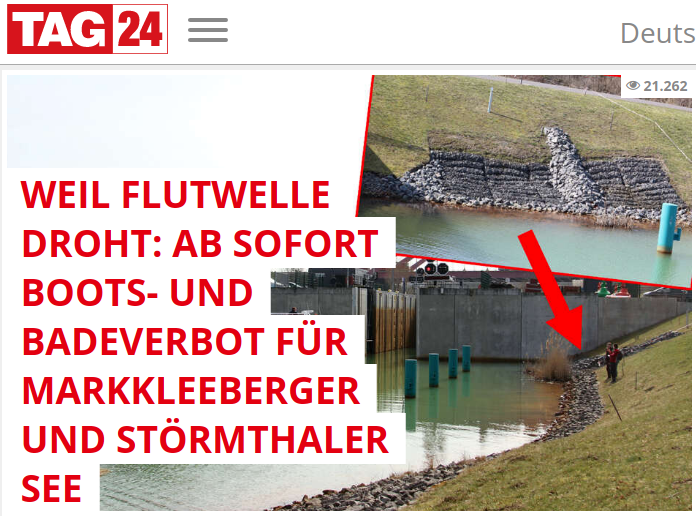
\includegraphics[width=0.62\textwidth]{fig_img/2021_03_25_tag24.png}
    \caption*{Böschung deformiert sich und droht abzurutschen \href{https://www.tag24.de/leipzig/lokales/hiobsbotschaft-ab-sofort-boots-und-badeverbot-fuer-markkleeberger-und-stoermthaler-see-1895366}{[Tag24]}
    }  
    \label{fig:markkleeberg}
\end{figure}
}

\only<2>{
\begin{center} \Large
\vfill

    Ein Blick auf \textbf{YouTube} u.ä. lohnt sich (Stichwörter: \textsl{Erdbeben/Earthquake, Bodendynamik/Soil Dynamics, \dots}). 
    
\vfill


\includegraphics[width=0.2\textwidth]{fig_img/youtube.png}
    
\end{center}
}

\end{frame}

\begin{frame}
\frametitle{Auslegung \& Bau}

\only<1>{
\begin{figure}
    \centering
    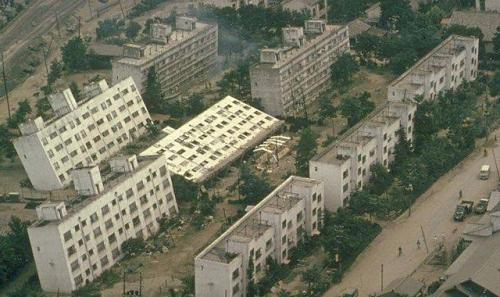
\includegraphics[width=0.81\textwidth]{fig_img/wikipedia_org_earthquake.jpeg}
    \caption*{Erdbeben \& Bodenverflüssigung \href{https://en.wikipedia.org/wiki/1964_Niigata_earthquake}{[Wikipedia]}}
    \label{fig:erdbeben}
\end{figure}
}

\only<2>{
\begin{figure}
    \centering
    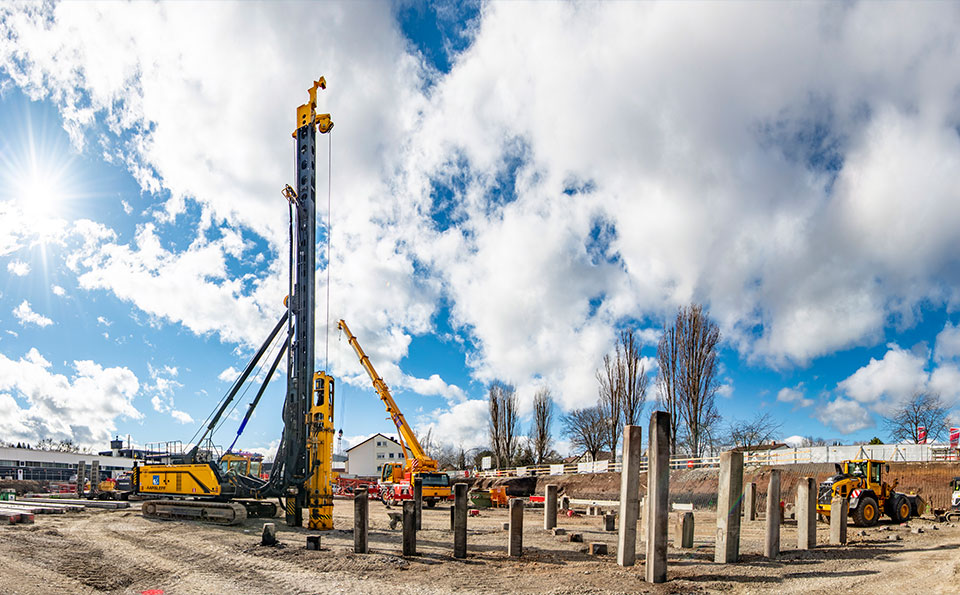
\includegraphics[width=0.75\textwidth]{fig_img/aarsleff_de_gruendung.jpg}
    \caption*{Gründungen und Fundamente \href{https://www.aarsleff-grundbau.de/media/wissenswertes/allgemeines/pfahlgruendung/}{[Aarsleff]}}
    \label{fig:gruendung}
\end{figure}
}

\only<3>{
\begin{figure}
    \centering
    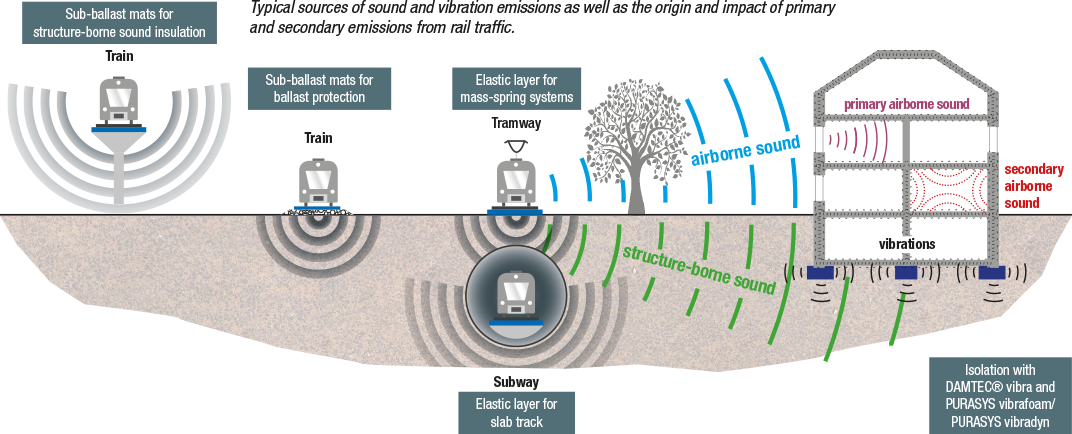
\includegraphics[width=\textwidth]{fig_img/kraiburg_purasys_com_isolation.png}
    \caption*{Erschütterungsschutz, urban noise \href{https://www.kraiburg-purasys.com/en/acoustic-vibration-isolation-rail-traffic/}{[Kraiburg-Pyrasys]}}
    \label{fig:erschuetterung}
\end{figure}
}

\only<4>{
\begin{figure}
    \centering
    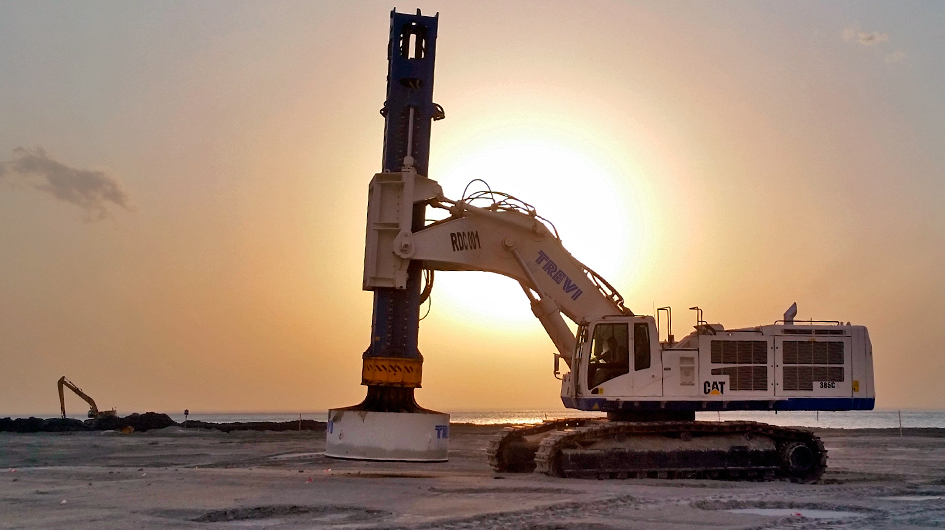
\includegraphics[height=0.615\textheight]{fig_img/treviaustria_eu_verdichtung.jpg}
    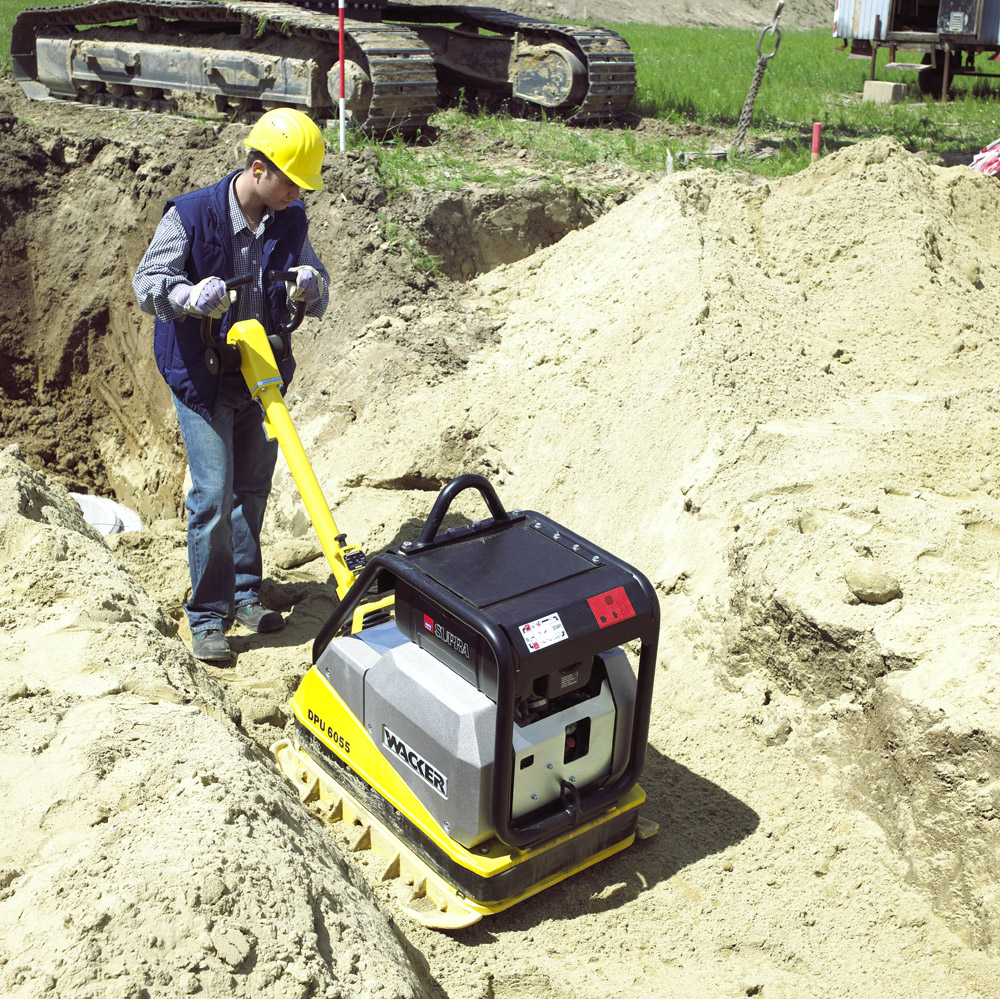
\includegraphics[height=0.615\textheight]{fig_img/wikipedia_org_ruettelplatte.jpg}
    \caption*{Bodenverdichtung und Bodenverbesserung
    \href{https://www.treviaustria.eu/technologien/dynamische-intensivverdichtung}{[TREVI Geotechnik]}, \href{https://de.wikipedia.org/wiki/Rüttelplatte}{[Wikipedia]}}
    \label{fig:verdichtung}
\end{figure}
}
% Rütteldruckverdichtung, Rüttelstopfverdichtung, Sprengverdichtung

\only<5>{
\begin{figure}
    \centering
    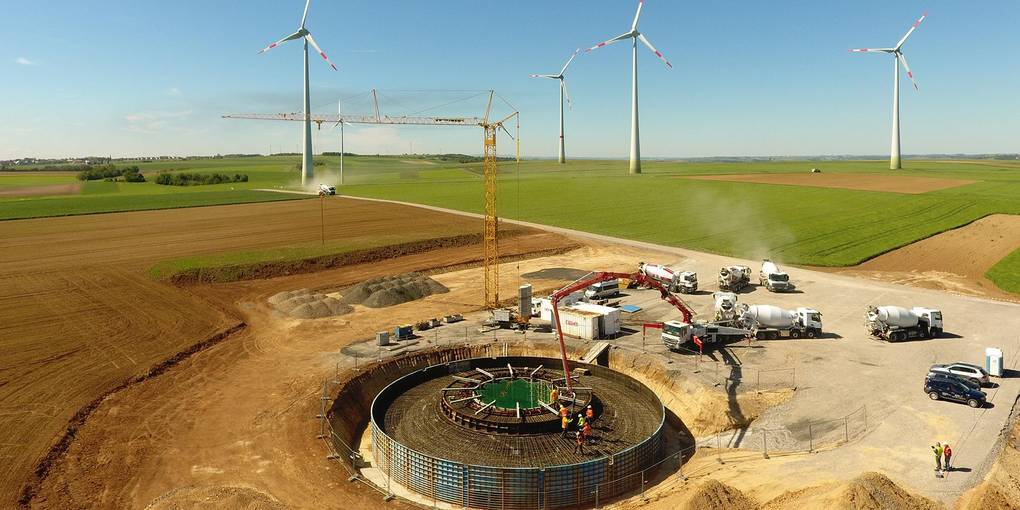
\includegraphics[width=0.95\textwidth]{fig_img/allgemeine_zeitung_de_windkraft.jpg}
    \caption*{Windkraft \href{https://www.allgemeine-zeitung.de/lokales/mainz/stadtteile-mainz/hechtsheim/windrad-mit-2295-metern-hohe-in-mainz-hechtsheim_20190020}{[Allgemeine Zeitung]}}
    \label{fig:windlasten}
\end{figure}
}

\end{frame}

\begin{frame}
\frametitle{Analyse \& Bewertung}

\only<1>{
\begin{figure}
    \centering
    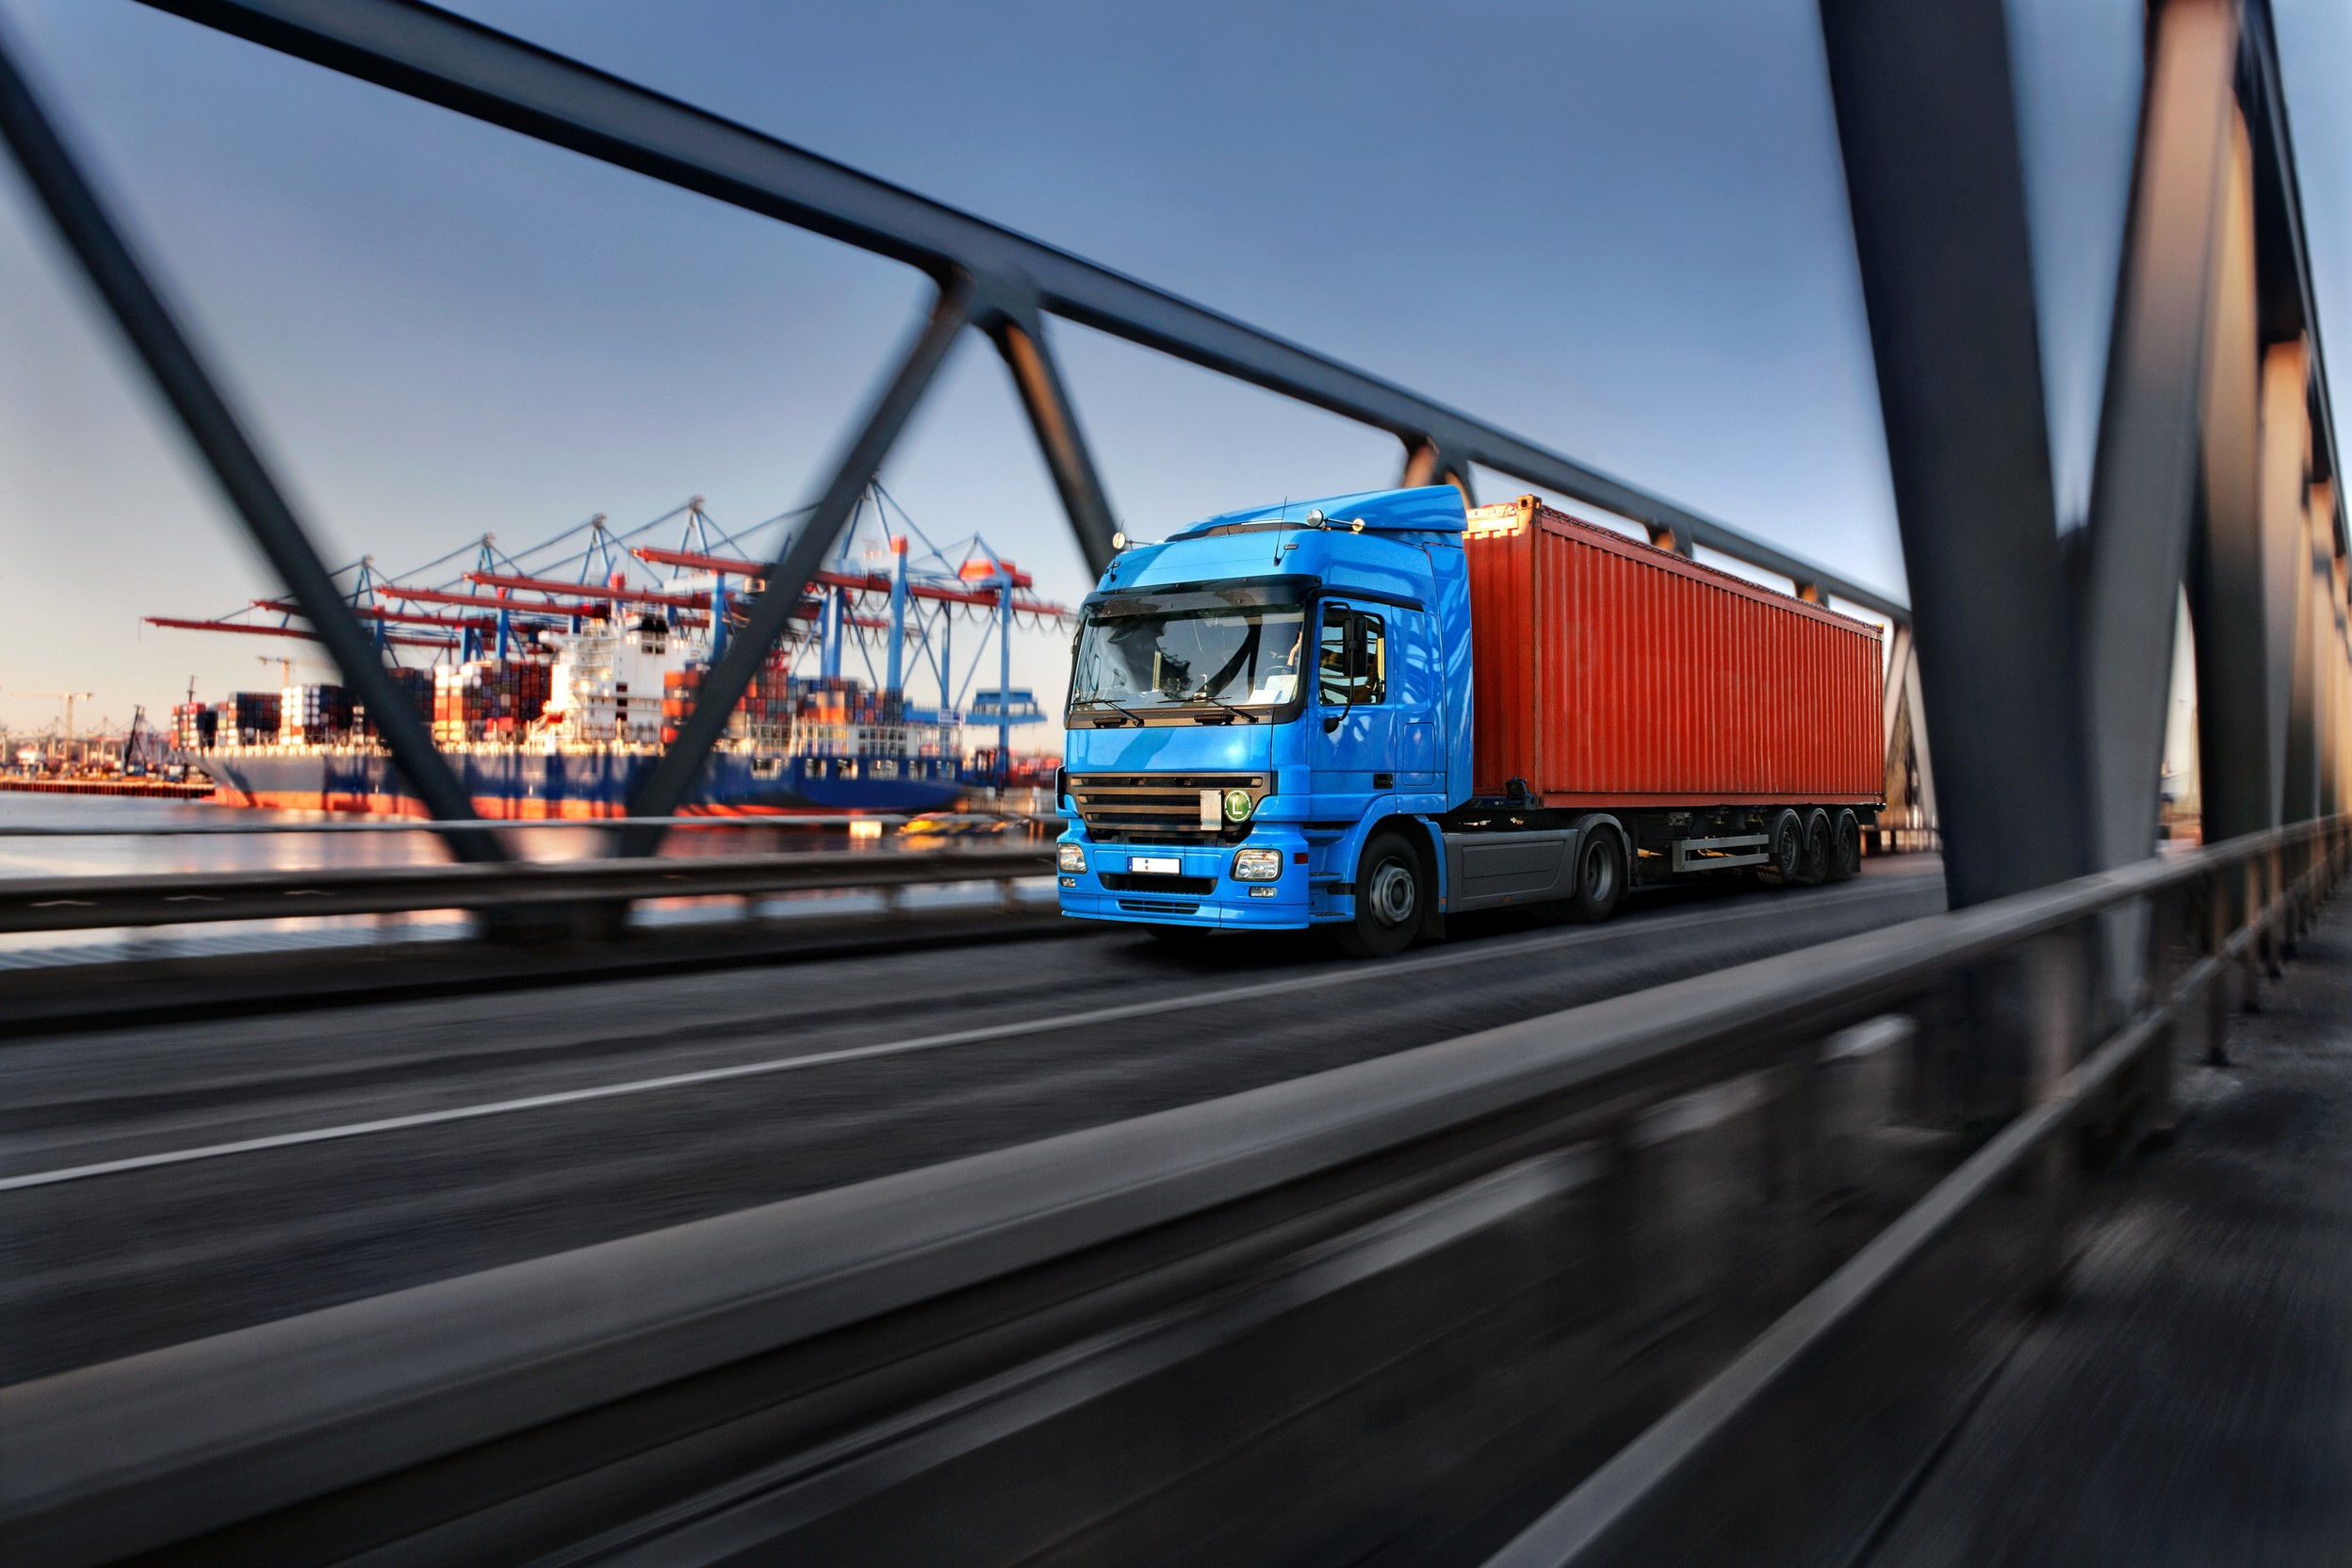
\includegraphics[width=0.74\textwidth]{fig_img/daudyn_com_verkehr.jpg}
    \caption*{Verkehr \href{https://www.baudyn.de/referenzen/strassenverkehr/}{[BauDyn]}}
    \label{fig:verkehr}
\end{figure}
}

\only<2>{
\begin{figure}
    \centering
    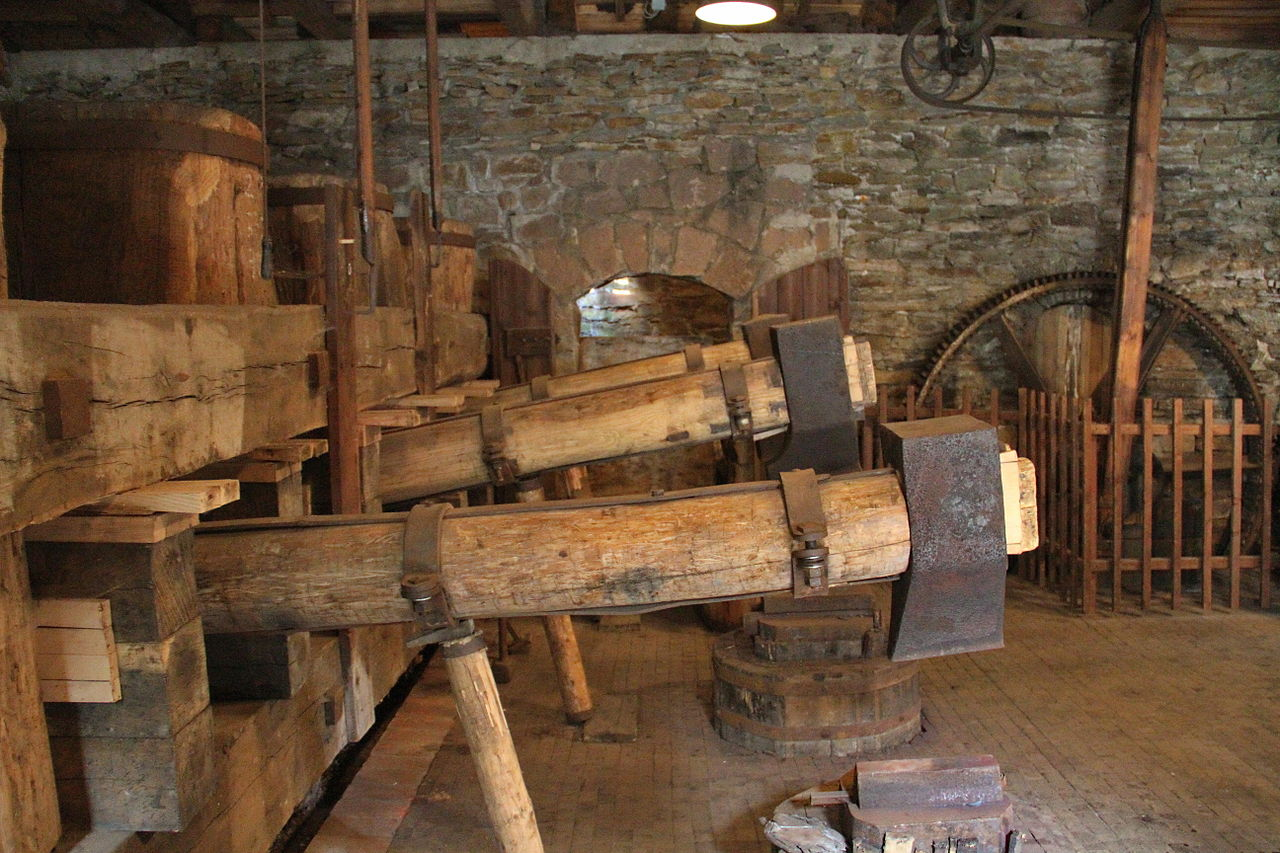
\includegraphics[width=0.72\textwidth]{fig_img/wikipedia_org_freiberger_hammer.jpeg}
        \caption*{Produktionsstätten
    \href{https://de.wikipedia.org/wiki/Freibergsdorfer_Hammer}{[Wikipedia]}} 
    \label{fig:industrie}
\end{figure}
}

\only<3>{
\begin{figure}
    \centering
    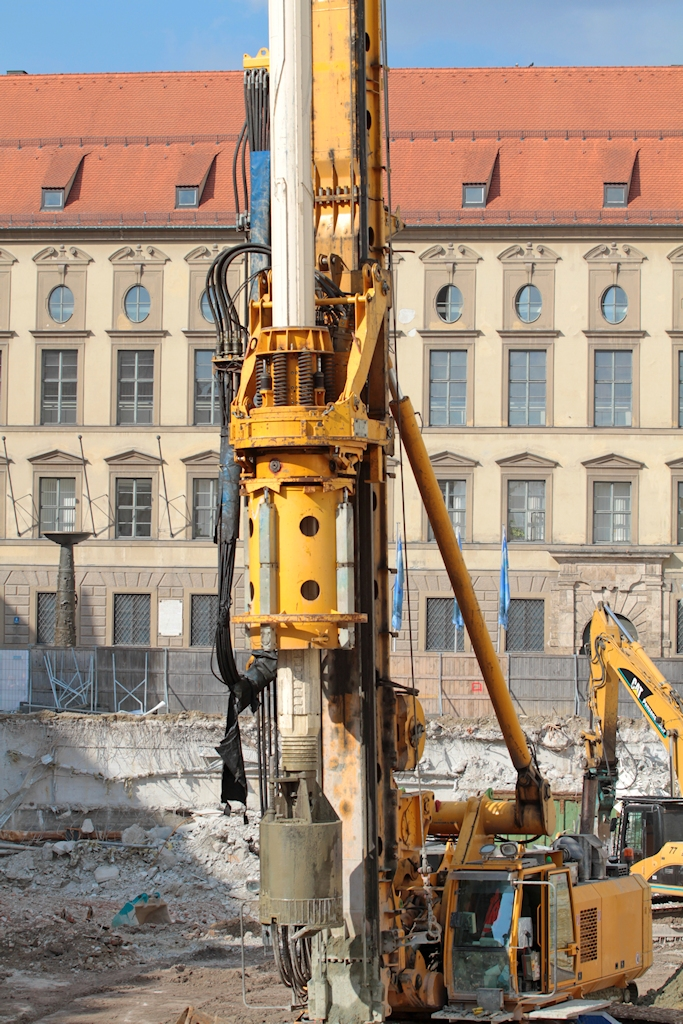
\includegraphics[height=0.85\textheight]{fig_img/lga_de_bauramme.jpg}
    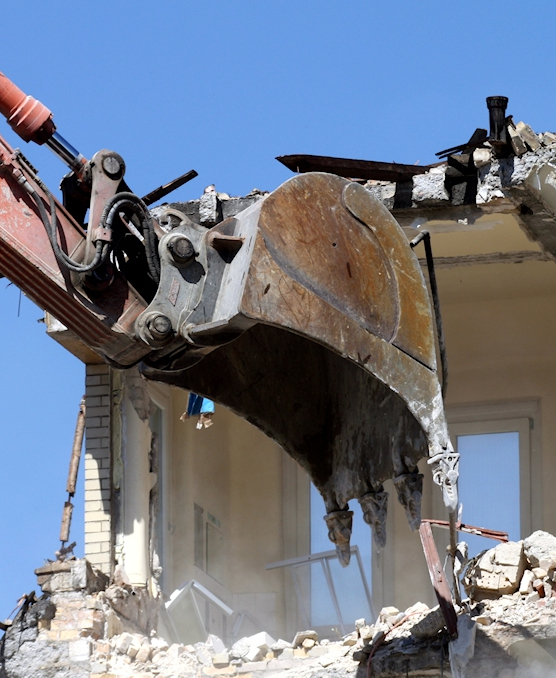
\includegraphics[height=0.85\textheight]{fig_img/lga_de_bagger.jpg}
    \caption*{Bauarbeiten \href{https://www.lga.de/en/dienstleistungen/erschuetterungsschutz-nach-din-4150/}{[LGA]}}
    \label{fig:bauarbeiten}
\end{figure}
}

\only<4>{
\begin{figure}
    \centering
    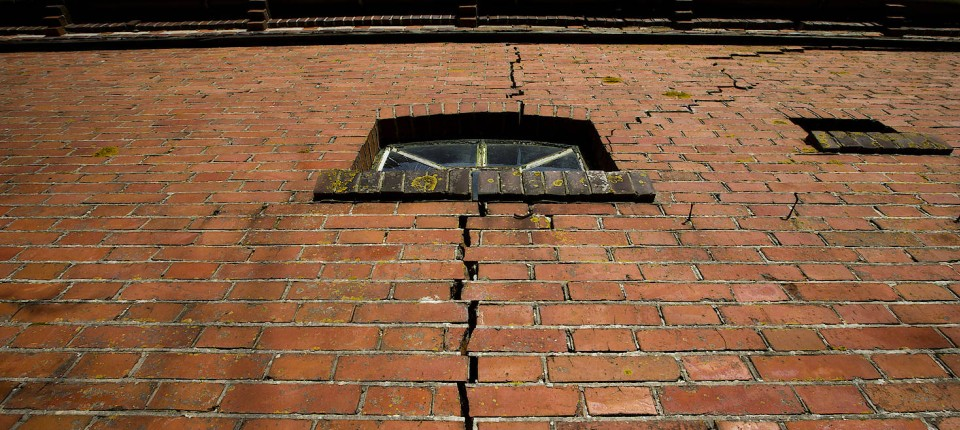
\includegraphics[width=\textwidth]{fig_img/faz_net_riss.jpg}
    \caption*{Gebäudeschäden \href{https://www.faz.net/aktuell/gesellschaft/ungluecke/erschuetterungen-in-den-niederlanden-fuehren-zu-debatte-ueber-erdgasfoerderung-16201165.html}{[FAZ]}}
    \label{fig:schaeden}
\end{figure}
}

\only<5>{
\begin{figure}
    \centering
    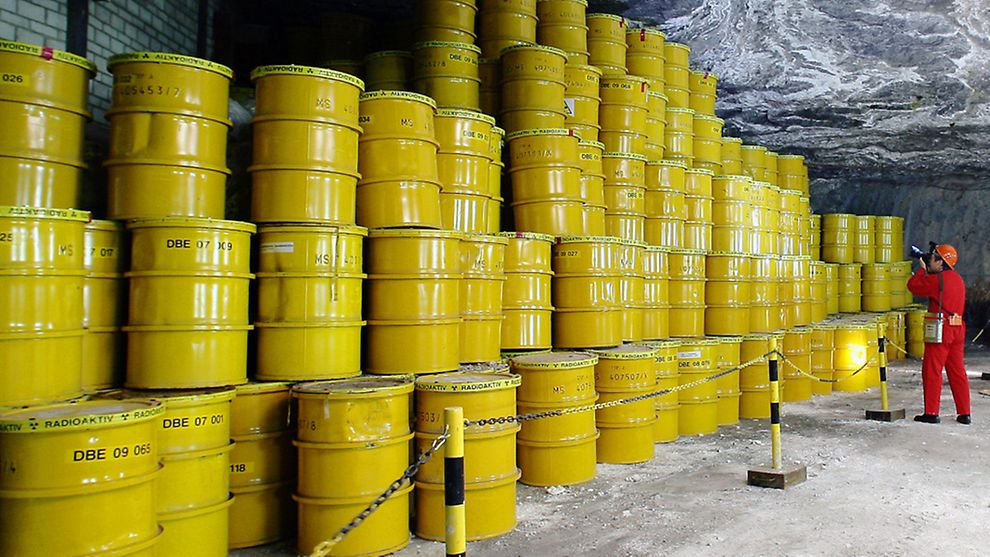
\includegraphics[width=0.85\textwidth]{fig_img/bundesregierung_de_endlager.jpg}
    \caption*{Endlager \href{https://www.bundesregierung.de/breg-de/aktuelles/endlagergesetz-in-kraft-getreten-394898}{[Bundesregierung]}}
    \label{fig:endlager}
\end{figure}
}

\end{frame}

\begin{frame}
\frametitle{Erkundung und Überwachung}

\only<1>{
\begin{figure}
    \centering
    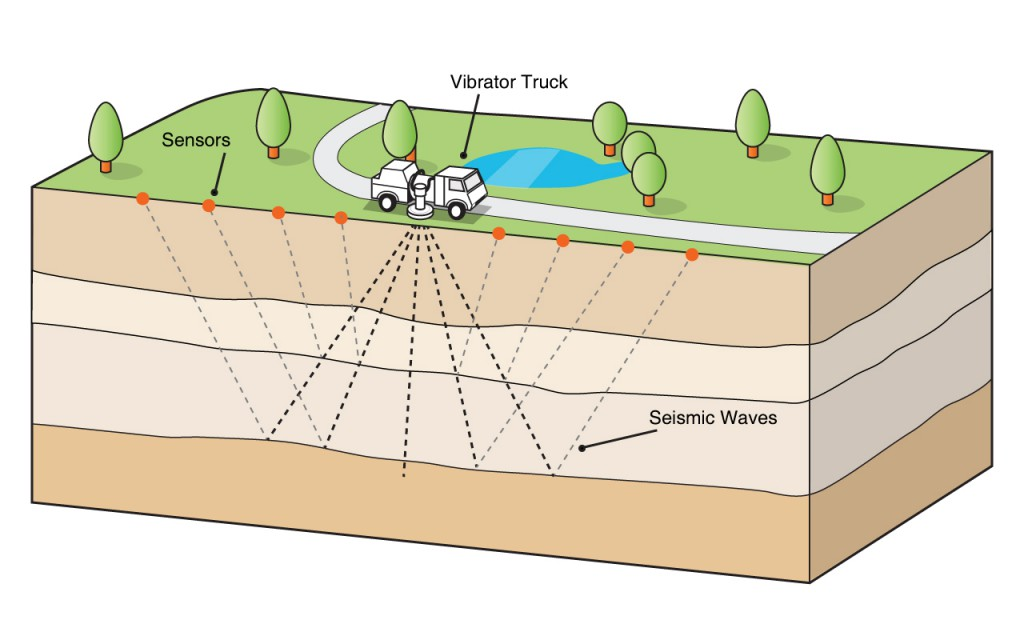
\includegraphics[width=0.76\textwidth]{fig_img/innoseis_com_exploration.jpg}
        \caption*{Bodenkennwertermittlung
    \href{http://www.innoseis.com/seismic-surveying/}{[innoseis]}} 
    \label{fig:feldversuch}
\end{figure}
}

\only<2>{
\begin{figure}
    \centering
    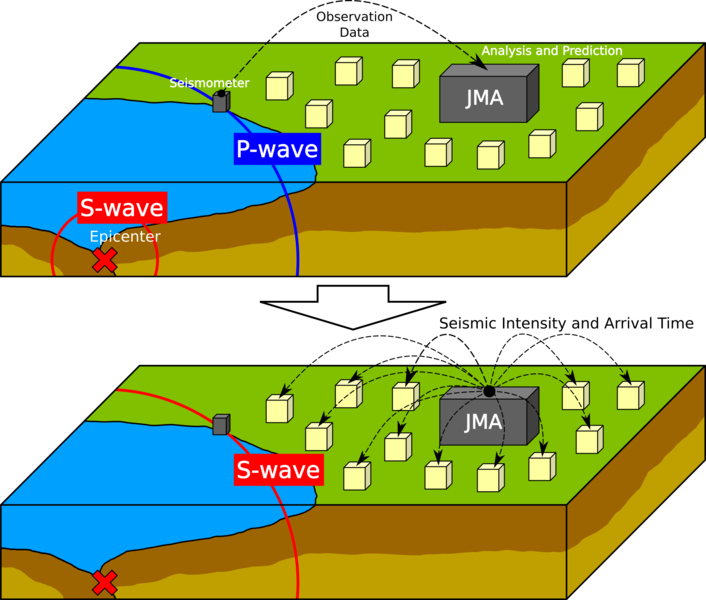
\includegraphics[width=0.56\textwidth]{fig_img/wikipedia_org_monitoring.png}
    \caption*{Erdbebenfrühwarnsystem \href{https://en.wikipedia.org/wiki/Earthquake_Early_Warning_(Japan)}{[Wikipedia]}}
    \label{fig:monitoring}
\end{figure}
}

\end{frame}


\begin{frame}
 \frametitle{Übersicht}
 \begin{enumerate}
  \item Einleitung
  \item Grundlagen
  \begin{enumerate}
  \item Einfreiheitsgradschwingungen %(frei, erzwungen)
  \item Frequenzanalyse
  \item Mechanisches Bodenverhalten %unter zyklischer Belastung
  \end{enumerate}
  \item Wellenausbreitung im Untergrund
  \begin{enumerate}
  \item Dehnstabsmodell (1D)
  \item Elastisches dreidimensionales Kontinuum (3D) %(Oberflächenwellen)
  \end{enumerate}
  \item Praktische Anwendung
  \begin{enumerate}
  \item Schwingungsmessung und Kennwertermittlung % Böden
  \item Erschütterungseinwirkungen % auf Menschen und Bauwerke
  \item Konstruktionskriterien % Erdbebensicheres Bauen
  \end{enumerate}
  \item Ausblick
  \end{enumerate}

  
  
\end{frame}


\begin{frame}
\frametitle{Organisatorisches}
    \begin{itemize}
        \item Vorlesung (online)
        \begin{itemize}
         \item angelehnt an \textsl{\cite{Verruijt2010, Vrettos2017, Schmidt2017}}
        \end{itemize}
        
        \item Übung
                \begin{itemize} 
                \item Vorrechnen ist Teil der Vorlesungen
                \item Hausaufgaben zum Selbstrechnen
                \item Diskussion der Lösungen anhand von \textsl{Jupyter-Notebooks} (\textsl{Python})
        \end{itemize}

        \item Klausur (online)
        \begin{itemize}
         \item schriftlich, 120 Minuten
         \item Datum und Details folgen
        \end{itemize}
    \end{itemize}

\end{frame}
%%%%%%%%%%%%%%%%%%%%%%%%%%%%%%%%%%%%%%%%%%%%%%%%

\section*{Literaturverzeichnis}

\begin{frame}[allowframebreaks]{}
	\printbibliography
\end{frame}

\end{document}
